\chapter{Arquitectura y herramientas} \label{arquitecturayh}
El proceso de diseñar es definido por el IEEE como el esfuerzo para definir la arquitectura, componentes, interfaces y otras características de un sistema o componente. También se podría definir como la etapa del ciclo de vida del software en la cual se produce una descripción de la estructura interna del software que sirve de base para su construcción. El estándar ISO 12207 identifica un diseño a alto nivel o arquitectónico y un diseño detallado. El primero describe la estructura y organización, es decir, los subsistemas o componentes y sus relaciones. El segundo, describe cada componente y su comportamiento específico, para proceder a su construcción.

Después de tener una idea formada de los objetivos y requisitos del presente proyecto, en este capítulo nos centraremos en el diseño de alto nivel o la arquitectura, donde además de utilizar representaciones gráficas a alto nivel del sistema se detallarán las tecnologías y elementos arquitectónicos básicos del mismo, así como las herramientas utilizadas para llevar a cabo el proyecto.

\section{Arquitectura del sistema} \label{arquitectura}
Analizando los requisitos y los objetivos del proyecto se identifican tres partes críticas en el sistema: la interfaz gráfica de usuario (interfaz web), el API de los servicios web de los test estadísticos y el módulo STAC (\textit{Statistical Tests for Algorithm Comparison}), donde están incluidos los propios test estadísticos (tanto los test paramétricos como los test no paramétricos). En la figura \ref{fig:arquitectura} podemos ver la arquitectura de la plataforma web:

\begin{figure}[H]
\centering
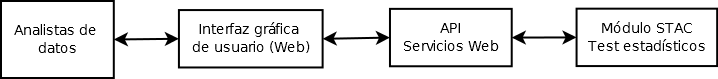
\includegraphics[width=15cm]{figuras/arquitectura.png}
\caption{Arquitectura de la plataforma web.}
\label{fig:arquitectura}
\end{figure}

Como podemos ver, los usuarios están representados como analistas de datos, y hacen uso de la interfaz gráfica de usuario (interfaz web), donde pueden realizar tareas tales como subir sus resultados y visualizarlos para posteriormente poder aplicar sobre ellos alguno de los test disponibles en el sistema. Esta interfaz representa la cara visible hacia el usuario, y por tanto será lo más usable posible para facilitar la tarea de validación.

La interfaz gráfica a su vez se comunica con el API de los servicios web, que son los encargados de ejecutar los test estadísticos con los parámetros u opciones elegidas por el analista en la interfaz (nivel de significancia, etc.), y devolver los datos obtenidos por el test a la interfaz para que ésta represente los datos de la forma más cómoda posible.

Por último, la parte más importante de la plataforma está representada por el módulo STAC, compuesto tanto por test paramétricos como no paramétricos. Aquí el usuario dispone de varios test, entre los que se encuentran por ejemplo aquellos que verifican si se cumplen las condiciones de homocedasticidad o normalidad para determinar si se pueden aplicar con seguridad (fiabilidad) test paramétricos.

Con el objetivo de desacoplar los datos y la lógica de negocio (modelo) de la interfaz de usuario (vista) y el módulo encargado de gestionar los eventos (controlador), se ha aplicado el patrón MVC (Modelo-vista-controlador) para construir la plataforma web. El concepto de patrón de diseño se explicará en más profundidad en secciones posteriores. En la figura \ref{fig:mvc} se muestra una representación gráfica de esta arquitectura, que ha sido en la que se ha basado este proyecto y en la que se distinguen las siguientes partes:

\begin{figure}[H]
\centering
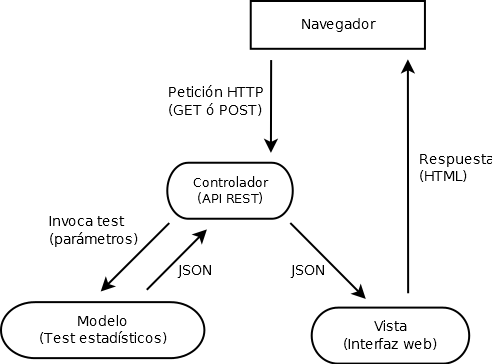
\includegraphics[width=9cm]{figuras/mvc.png}
\caption{Patrón MVC.}
\label{fig:mvc}
\end{figure}

\begin{itemize}
\item El controlador se encarga de recibir las peticiones HTTP (GET o POST) del navegador y decide qué test estadístico quiere invocar (para lo cual realizará una llamada con ciertos parámetros). La subida y visualización de ficheros de datos son tratados por el propio controlador. Éste una vez obtenga los datos se los devolverá a la vista (en formato JSON). En este proyecto el controlador está representado por el API de servicios web REST.
\item Las vistas reciben los datos del modelo a través del controlador y se los muestran a los usuarios (en formato HTML), en ellas únicamente se realizan operaciones simples. Representa la interfaz gráfica de usuario (Web).
\item El modelo es el responsable de realizar una gran parte de las funcionalidades del sistema, ya que en él se lleva a cabo la realización de las distintas pruebas de hipótesis. Esta parte representaría al módulo STAC, en donde se localizan los test paramétricos y no paramétricos.
\end{itemize}

Las tecnologías mencionadas (HTTP, REST, JSON) se detallan en secciones posteriores dentro del presente capítulo.

\section{Herramientas de diseño}
En este proyecto se utiliza la programación modular como paradigma de programación. La programación modular consiste en dividir un programa en módulos o subprogramas con el fin de hacerlo más legible y manejable. Un módulo es cada una de las partes de un programa que resuelve uno de los subproblemas en que se divide el problema complejo original. Cada uno de estos módulos tiene una tarea bien definida y algunos necesitan de otros para poder operar. La razón de realizarlo de esta forma y no orientado a objetos es debido a que los test estadísticos implementados son funciones en sí, los cuales reciben una serie de parámetros y devuelven unos resultados. Para el caso de la API REST, el framework elegido que se verá en secciones posteriores hace también que los servicios web tengan una representación en forma de función, con lo que sería añadir una complejidad extra al proyecto innecesaria.

Para poder modelar el software de un modo formal se utilizará UML (\textit{Unified Modeling Language}). UML es un lenguaje gráfico para visualizar, especificar y documentar cada una de las partes que comprende el desarrollo de software. Permite especificar diferentes ámbitos del sistema desde la lógica de negocio hasta la estructura hardware, sin ligarse a ningún lenguaje de desarrollo en particular. Para ello, hace uso de modelos que representan el sistema desde un punto de vista específico.

UML proporciona 13 tipos de diagramas, que se dividen en tres categorías: estructura, comportamiento e interacción. Pese a que UML está por lo general ligado a la programación orientada a objetos, en este proyecto se utilizará para realizar un diagrama de la categoría de interacción, que servirá para definir acciones que se pueden realizar en la plataforma:

\noindent
\begin{itemize}
\item \textbf{Diagramas de secuencia:} indican los componentes que forman parte del sistema y las llamadas que se hacen en cada uno de ellos para realizar una tarea determinada. Los mensajes o llamadas intercambiados están ordenados temporalmente (en secuencia).
\end{itemize}

\subsection{Herramientas}
Para poder realizar los diagramas UML y el prototipo de la interfaz gráfica del usuario, se han utilizado las siguientes herramientas:

\begin{itemize}
\item \textbf{StarUML:} herramienta que soporta la mayoría de los tipos de diagramas especificados en UML 2.0 y que servirá para realizar los diagramas en este proyecto.
\item \textbf{Lumzy:} herramienta de creación de prototipos para sitios web y aplicaciones.
\end{itemize}

\subsection{Patrones de diseño}
Un patrón es una solución a un problema en un contexto particular. Es recurrente (lo que hace la solución relevante a otras situaciones), enseña (permite entender cómo adaptarlo a la variante particular del problema donde se quiere aplicar) y tiene un nombre para referirse al patrón. Los patrones facilitan la reutilización de diseños y arquitecturas software que han tenido éxito. Existen tres categorías de patrones de diseño:
\begin{itemize}
\item \textbf{Patrones de creación:} tratan de la inicialización y configuración de clases y objetos.
\item \textbf{Patrones estructurales:} tratan de desacoplar interfaz e implementación de clases y objetos.
\item \textbf{Patrones de comportamiento:} tratan de las interacciones dinámicas entre sociedades de clases y objetos.
\end{itemize}

Debido a que los patrones de diseño están fuertemente ligados al paradigma orientado a objetos (clases y objetos), en este proyecto se utilizan solamente dos patrones:
\begin{itemize}
\item \textbf{El patrón MVC:} visto en la sección \ref{arquitectura}, encaja dentro de los denominados patrones estructurales, y sirve para desacoplar interfaz e implementación
\item \textbf{El patrón \textit{Singleton} (Fig. \ref{fig:singleton}):} para la implementación de la historia de usuario \textbf{HU-5} vista en la sección \ref{hu_desarrollador}. Este es el único punto del proyecto donde se utiliza programación orientada a objetos. La razón de utilizar una clase para implementar la \textbf{HU-5} en este caso se facilita la programación de esta característica del proyecto.
\end{itemize}

\noindent
\textbf{Patrón Singleton}

Este patrón está diseñado para restringir la creación de objetos pertenecientes a una clase o el valor de un tipo a un único objeto. Su intención consiste en garantizar que una clase sólo tenga una instancia y proporcionar un punto de acceso global a ella (Fig. \ref{fig:singleton}). El patrón \textit{singleton} se implementa creando en nuestra clase un método que crea una instancia del objeto sólo si todavía no existe alguna. Para asegurar que la clase no puede ser instanciada nuevamente se regula el alcance del constructor (con atributos como protegido o privado).

\begin{figure}[H]
\centering
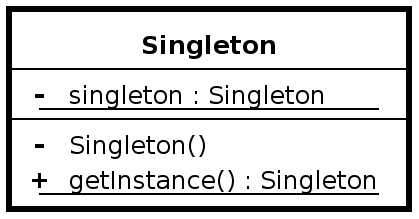
\includegraphics[width=6cm,height=3cm]{figuras/singleton.png}
\caption{Patrón \textit{Singleton}.}
\label{fig:singleton}
\end{figure}

\section{Herramientas de desarrollo}

\subsection{Análisis de librerías de test estadísticos en Python} \label{libreriastest}

\subsubsection{\textbf{Librería SciPy - \textit{Scientific Computing Tools for Python}}}
SciPy \cite{scipy} cuenta con una colección denominada \textit{The SciPy Stack}, que consta de un conjunto de paquetes principales de software de código abierto para la computación científica en Python, donde la comunidad puede utilizar y desarrollar esta colección. Entre los paquetes básicos de esta colección se encuentran:
\begin{itemize}
\item \textbf{NumPy:} paquete fundamental para computación numérica, donde se puede encontrar álgebra lineal, operaciones estadísticas básicas (como la media, la varianza, ...), aleatoriedad, etc. 
\item \textbf{Librería SciPy:} una colección de algoritmos numéricos y herramientas específicas de dominio, incluyendo el procesamiento de señales, la optimización, estadística, etc.
\end{itemize}
SciPy y NumPy tienen versiones de documentación en formato HTML y PDF \cite{scipy-doc}, que cubren casi toda la funcionalidad disponible.
La librería SciPy es uno de los paquetes principales que componen \textit{The SciPy Stack}. Proporciona muchas rutinas numéricas fáciles de usar y eficientes, como las rutinas de integración numérica y optimización. SciPy está organizada en subpaquetes o módulos que cubren diferentes dominios de computación científica. Para este proyecto, el subpaquete que nos interesa es \textit{\textbf{stats}}, que consta de distribuciones y funciones estadísticas.

El subpaquete \textit{stats} contiene un gran número de distribuciones de probabilidad (tanto continuas como discretas). Las continuas (como la distribución $\chi^2$ ó $\mathcal{T}$ vistas en la sección \ref{estadistico}) son las que nos interesan. Estas distribuciones continuas definidas como clases constan de métodos comunes, como son la función de densidad de probabilidad o la función de distribución acumulada para una distribución determinada, de las que ya hemos hablado en la figura \ref{fig:comparativa_pdf_cdf}. Estas funciones sirven de utilidad para realizar los test estadísticos y obtener valores necesarios. Así mismo, este módulo proporciona también una biblioteca de test estadísticos. Entre estos test están aquellos para hallar las condiciones paramétricas de normalidad (Shapiro-Wilk, D’Agostino–Pearson y Kolmogorov–Smirnov), y homocedasticidad (Levene), así como la prueba $\mathcal{T}$ de Student (vistos en la sección \ref{parametricos} del capítulo \ref{contraste}). 

Un módulo de la librería SciPy se define como un subpaquete Python del paquete SciPy: scipy/subpaquete. Este subpaquete contiene los archivos de Python con el código de las diferentes funcionalidades, así como aquellos archivos de inicialización e importación que sirven para facilitar su uso.

Por tanto, para este proyecto nos serviremos de los test de las condiciones paramétricas, así como de la prueba $\mathcal{T}$ de Student incluidos en esta librería, ya que forman parte de los objetivos del proyecto. Sin embargo, esta librería no cubre todas las necesidades de test detalladas en los objetivos para el proyecto.
 
\subsubsection{\textbf{Librería nonparametric.py}} \label{nonparametric}
Este módulo, creado por Ismael Rodríguez, contiene algunos de los test marcados como objetivos en este proyecto: el test de Wilcoxon, el test de Friedman, el test de Iman-Davenport, el test de Bonferroni-Dunn, el test de Holm y el test Hochberg. Sin embargo, no se ha probado su correcto funcionamiento y por tanto algunos de ellos necesitarán ser rediseñados e implementados de nuevo. Para ello será necesario:

\begin{itemize}
\item Probar que funcionan correctamente mediante la realización de test unitarios y corregir los fallos encontrados.
\item Comprobar que devuelven los datos necesarios: rankings, estadísticos, $\textit{p-valor}$ (en caso de los test de ranking); y los parámetros usados para cada comparación, $\textit{p-valor}es$ ajustados (en el caso de los test de comparación).
\item Hacer que reciban y devuelvan los datos de la misma manera. 
\end{itemize}

Este módulo tiene dependencias con la librería SciPy (con el módulo \textit{stats}), así como con el paquete NumPy. Como se ha dicho anteriormente, la funcionalidad de SciPy sirve a este proyecto para poder hallar parámetros básicos que serán necesarios para obtener todos los datos necesarios en los test.

Dado que será necesario corregir y volver a implementar muchas de las funcionalidades presentes en este módulo, y debido a que muchas otras funcionalidades aún quedan por implementar, este módulo tampoco cumple con las expectativas del proyecto. La extensión y corrección de este módulo permitirá la obtención de un módulo acorde a los objetivos del proyecto con todos los test disponibles. 

\subsection{Análisis de librerías para servicios REST en Python} \label{bottle}

\subsubsection{\textbf{Servicios REST}}
Los test estadísticos, así como la subida y consulta de ficheros serán accesibles vía web mediante servicios web en Python y basados en REST. La Transferencia de Estado Representacional (\textit{Representational State Transfer}) o REST es una técnica de arquitectura software para sistemas hipermedia distribuidos como la World Wide Web. El término se originó en el año 2000, en una tesis doctoral sobre la web escrita por Roy Fielding, uno de los principales autores de la especificación del protocolo HTTP y ha pasado a ser ampliamente utilizado por la comunidad de desarrollo. Aunque REST no es un estándar, está basado en los estándares: HTTP, URL, representación de los recursos (XML, HTML, GIF, JPEG, JSON ...), y tipos MIME (text/xml, text/html, application/json, ...)

Por ejemplo, en la figura \ref{fig:rest} se puede ver como ejemplo una petición para consultar el contenido de un archivo. Para ello, la respuesta indica en la cabecera con ``Content-Type: application/json", el tipo de dato a devolver, por lo que el cliente sabe que el contenido de la respuesta es una cadena en formato JSON, y puede procesarla como prefiera. Los servicios web REST están basados en los siguientes principios:

\begin{itemize}
\item \textbf{Utilización de métodos HTTP:} por tanto, los métodos a utilizar para la comunicación con los servicios web de los test podrán ser los comunes de HTTP: GET, POST, PUT, DELETE.
\item \textbf{Servicios sin estado:} las peticiones a los servicios web de los test incluirán todos los datos necesarios (petición completa e independiente) para que el servidor no tenga que mantener ningún estado para procesar la petición. En otras palabras, el servidor no puede almacenar información proporcionada por el cliente en una solicitud y usarlo en otra solicitud.
\item \textbf{Exposición de URIs (identificador recursos uniforme) con forma de directorios:} por ejemplo, se podrían hacer URIs del estilo: http://localhost/api/nombre\_test/...
\end{itemize}

\begin{figure}[H]
\centering
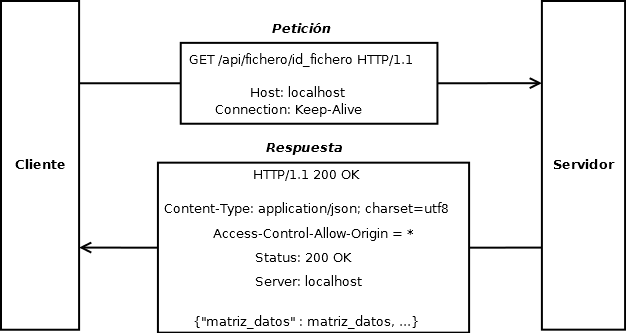
\includegraphics[width=12cm,height=6cm]{figuras/rest.png}
\caption{Servicios web REST.}
\label{fig:rest}
\end{figure}

Cabe destacar que para el presente proyecto se utilizarán los métodos HTTP GET y POST, el primero para obtener información de un recurso (esto es, obtener los resultados de los test, así como el contenido del fichero) y el segundo para crear un nuevo recurso (para la creación de un nuevo fichero). Así mismo, los recursos estarán representados por el tipo MIME ``application/json". La figura \ref{fig:rest} muestra estas características.

\subsubsection{\textbf{Librería Bottle}}
Para desarrollar los servicios web que diesen acceso a los test estadísticos, así como a la gestión del fichero, en el anteproyecto se había barajado la utilización de alguno de los siguientes frameworks: Flask, Web.py y Bottle. El framework elegido finalmente fue Bottle \cite{bottle}. Este framework web es conocido más bien como un micro framework, y las principales razones que propiciaron su elección frente a las demás es que se trata de un framework rápido, sencillo y ligero para Python. Se distribuye como un módulo y esta formado por un único archivo y no tiene dependencias distintas de la biblioteca estándar de Python. Además, dispone de las siguientes características:
\begin{itemize}
\item \textbf{Enrutamiento:} mapeo de solicitudes de llamadas a función con soporte para URLs limpias y dinámicas.
\item \textbf{Plantillas:} motor de plantillas integrado.
\item \textbf{Utilidades:} la facilidad de acceso a datos de formulario, subida de ficheros, cookies, cabeceras y otros metadatos relacionados con HTTP.
\item \textbf{Servidor:} servidor HTTP propio para desarrollo integrado y soporte para cualquier servidor HTTP compatible con la especificación WSGI (interfaz entre servidores web y aplicaciones web o frameworks para el lenguaje Python).
\end{itemize}

Bottle permite la implementación de servicios web accesibles mediante una o más URIs. El decorador \textit{route()} asigna una URI a un trozo de código (el propio servicio) en lo que se denomina ruta. El decorador decora a lo que realmente referencia, que es un trozo de código. Cada vez que el navegador llama a una URL especificada con \textit{route()} la función o servicio asociado es llamado y el valor de retorno se envía al navegador. A un mismo servicio se pueden unir tantas URIs como se desean. El siguiente código muestra cómo de una forma sencilla se puede implementar un servicio REST:

\begin{lstlisting}
@route('/fichero/<id_fichero>', method='GET')
def consultar_fichero(id_fichero):
    response.headers['Access-Control-Allow-Origin'] = '*'
    response.content_type = "application/json"
    ...
    return datos
\end{lstlisting}

Como se puede ver en ejemplo, por medio de \textit{@route} se indica la URL. El método utilizado en este caso es GET y la respuesta será dada en formato JSON. Con \textit{id\_fichero}, se indica que se va a pasar el identificador del fichero como parte de la URL.

\subsection{Análisis de frameworks para desarrollo web}

\subsubsection{\textbf{Twitter Bootstrap}}
El framework para el desarrollo de la interfaz web utilizado en la plataforma es Twitter Bootstrap \cite{bootstrap}. Bootstrap fue desarrollado por Mark Otto y Jacbod Thornton de Twitter, como solución interna para solucionar las inconsistencias en el desarrollo dentro del equipo de ingeniería de Twitter, ya que hasta ese momento no había establecida ninguna convención sobre las formas en las que los ingenieros desarrollaban la plataforma. En agosto del 2011, Twitter liberó a Bootstrap como código abierto. En febrero del 2012, se convirtió en el proyecto de desarrollo más popular de GitHub \cite{github} y es utilizado por organizaciones como la NASA.

Se trata de un framework o conjunto de herramientas de software libre para diseño de sitios y aplicaciones web (\textit{Front-end} o interfaz). Contiene plantillas de diseño con tipografía, formularios, botones, cuadros, menús de navegación y otros elementos de diseño basado en HTML5 y CSS3, así como, extensiones de JavaScript opcionales adicionales. Una de sus principales características es que utiliza LESS, que es una ampliación de las hojas de estilo CSS, pero a diferencia de estás, funciona como un lenguaje de programación, permitiendo el uso de variables, funciones, operaciones aritméticas, entre otras, para acelerar y enriquecer los estilos en un sitio web.

\begin{figure}[H]
\centering
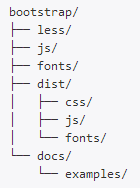
\includegraphics{figuras/bootstrap.png}
\caption{Organización Twitter Bootstrap.}
\label{fig:booststrap}
\end{figure}

La figura \ref{fig:booststrap} muestra la organización de directorios de Bootstrap. Los directorios less/, js/ y fonts/ contienen el código fuente utilizado para generar los archivos CSS, JavaScript y las fuentes. El directorio dist/ contiene los mismos archivos que se han mostrado en la sección anterior para la versión compilada de Bootstrap. El directorio docs/ incluye el código fuente de la documentación de Bootstrap y el directorio examples/, que contiene varios ejemplos de muestra. El resto de archivos incluidos proporcionan información de licencia y desarrollo.

Las razones de la utilización de este framework se basan en la sencillez y en la amplia documentación existente. Sin embargo, la razón principal es la capacidad para diseño \textit{responsive} o fluido (\textit{responsive design}). Mediante el diseño responsivo, se consigue que la web se adapte según según la resolución del dispositivo o ventana del navegador. Esto es necesario para poder desarrollar de un modo fácil y adecuado la historia de usuario \textbf{HU-5} vista en la sección \ref{hu_cliente} del capítulo \ref{analisisreq}. Para este propósito, Bootstrap cuenta con un diseño de páginas basado en rejillas, que están formadas por de filas y columnas donde se colocan los contenidos. Las rejillas crecen hasta 12 columnas a medida que crece el tamaño de la pantalla del dispositivo.

\subsection{Otras herramientas}
\subsubsection{\textbf{Desarrollo}}
Con el objetivo de disminuir los costes del proyecto, y teniendo en cuenta el uso de herramientas que requieran el menor tiempo de aprendizaje, el entorno de trabajo seleccionado para el desarrollo del proyecto fue el siguiente:
\begin{itemize}
\item \textbf{Sistema operativo:} Ubuntu 12.04, basado GNU/Linux.
\item \textbf{IDE de programación:} Spyder 2, entorno multiplataforma de código abierto para la programación científica en el lenguaje Python. La razón de su utilización es que Spyder integra NumPy y SciPy, entre otras librerías.
\end{itemize}
\subsubsection{\textbf{Documentación}}
Para el desarrollo de la documentación se han utilizado las siguientes herramientas:
\begin{itemize}
\item \textbf{Sphinx 1.2.2:} Sphinx se trata de una herramienta de código abierto para generación de documentación de código Python. Es utilizada para documentar el módulo de Python STAC perteneciente a los test estadísticos. La razón de su utilización es que permite la generación de documentación en formato HTML para poder acceder a ella desde el navegador. Además, permite la escritura de fórmulas mediante notación \LaTeX, lo cual es importante en este proyecto.
\item \textbf{TeXstudio 2.8.2:} IDE de código abierto de \LaTeX \space que proporciona un soporte moderno de escritura, corrección ortográfica interactiva, plegado de código y resaltado de sintaxis. Es utilizado para la realización de la documentación.
\item \textbf{ProjectLibre 1.5.9:} herramienta multiplataforma de código abierto utilizada para la elaboración de diagramas de Gantt.
\item \textbf{Dia 0.97.2:} herramienta multiplataforma de código abierto utilizada para la elaboración de diagramas en general. Es utilizada en este proyecto para elaborar el EDT, así como diagramas genéricos de arquitectura, etc.
\end{itemize}

\subsubsection{\textbf{Tecnologías}} \label{tecnologias}
A parte de las tecnologías anteriormente mencionadas, el desarrollo del proyecto también está marcado por la utilización de las siguientes otras:

\begin{itemize}
\item \textbf{HTML:} \textit{HyperText Markup Language}, hace referencia al lenguaje de marcado para la elaboración de páginas web. Es un estándar que, en sus diferentes versiones, define una estructura básica y un código para la definición de contenido de una página web, como texto, imágenes, etc.
\item \textbf{JavaScript:} es un lenguaje de programación interpretado. Se utiliza en páginas web HTML para realizar
operaciones en el marco de la aplicación cliente, sin acceso a funciones del servidor.
\item \textbf{CSS:} \textit{Cascading style sheets} u hojas de estilo en cascada es un lenguaje usado para definir la presentación de un documento estructurado escrito en HTML.
\item \textbf{Apache y el módulo WSGI:} a pesar de que el framework Bottle dispone de su propio servidor HTTP para desarrollo integrado, y aprovechando que soporta cualquier servidor HTTP compatible con la especificación WSGI, en este proyecto se optó por la utilización del servidor web Apache. La principal razón de realizarlo de este modo es que el tiempo de respuesta del servidor de Bottle era de 5 segundos cuando se accedía desde otra red, mientras que utilizando Apache se llega a bajar a 2-3 milisegundos. Además, con esto se consigue hacer disponible la API REST por el puerto 80.
\subitem \textbf{- Apache} es un servidor web HTTP de código abierto, que implementa el protocolo HTTP/1.12. Desde 1996, Apache es el servidor HTTP más usado. Alcanzó su máxima cuota de mercado en 2005 siendo el servidor empleado en el 70\% de los sitios web en Internet.
\subitem \textbf{- WSGI} es una interfaz o especificación entre servidores web y aplicaciones web o frameworks para el lenguaje Python. El módulo WSGI de Apache implementa la interfaz WSGI, lo cual permite servir las aplicaciones Python (nuestro caso el API REST).
\item \textbf{AJAX:} \textit{Asynchronous JavaScript} + XML, está formada varias por tecnologías que permiten realizar peticiones HTTP y modificaciones en las páginas de forma asíncrona sin necesidad de recargar la página. Entre los beneficios del uso de AJAX destaca la reducción del tráfico con el servidor. Es utilizada en este proyecto para poder llamar a los servicios REST y gestionar los datos devueltos por éstos (interacción con las páginas HTML).
\item \textbf{JSON:} \textit{JavaScript Object Notation}, es un formato ligero para el intercambio de datos. Es utilizado por AJAX y los servicios REST. La razón de la utilización de este formato es que puede ser interpretado por cualquier lenguaje (incluido Python). En la figura \ref{fig:rest} podemos ver un ejemplo de formato JSON en la respuesta a la petición.
\end{itemize}

\subsubsection{\textbf{Librerías}}
En la siguiente tabla se muestran las distintas librerías de JavaScript utilizadas en el desarrollo del proyecto:

\begin{table}[H]
	\centering
	\begin{tabular}{|l|c|c|}
		\hline
		\textbf{Librería} & \textbf{Versión} & \textbf{Página Oficial} \\ \hline
		jQuery & 1.11.0 & http://jquery.com/ \\ \hline
		MathJax & 2.4 & http://www.mathjax.org/ \\ \hline
	\end{tabular}
\end{table}

\begin{itemize}
\item \textbf{jQuery:} es una biblioteca de JavaScript que permite simplificar la manera de interactuar con los documentos HTML, manipular el árbol DOM, manejar eventos, desarrollar animaciones y agregar interacción con la técnica AJAX a páginas web. Es utilizada en este proyecto para trabajar junto con el framework Bootstrap y para realizar las llamadas AJAX a los servicios web.
\item \textbf{MathJax:} es un motor de visualización de código libre de JavaScript que permite visualizar fórmulas matemáticas en navegadores web, utilizando diferentes lenguajes de marcado (entre ellos \LaTeX). MathJax tiene licencia libre y funciona en todos los navegadores modernos. La razón de su utilización en el proyecto es que en alguna ocasión se necesita escribir fórmulas en documentos HTML, y esta librería constituye una manera fácil de llevar a cabo esta tarea.
\end{itemize}